%%%%%%%% ICML 2021 EXAMPLE LATEX SUBMISSION FILE %%%%%%%%%%%%%%%%%

\documentclass{article}

% Recommended, but optional, packages for figures and better typesetting:
\usepackage{microtype}
\usepackage{graphicx}
\usepackage{subfigure}
\usepackage{booktabs} % for professional tables
\usepackage{multirow}
% hyperref makes hyperlinks in the resulting PDF.
% If your build breaks (sometimes temporarily if a hyperlink spans a page)
% please comment out the following usepackage line and replace
% \usepackage{icml2021} with \usepackage[nohyperref]{icml2021} above.
\usepackage{hyperref}
\usepackage{caption}
\usepackage{subcaption}
\usepackage{listings}

% Attempt to make hyperref and algorithmic work together better:
\newcommand{\theHalgorithm}{\arabic{algorithm}}

\usepackage[accepted]{icml2021}

% The Impact of Edge Detection on Sign Language Alphabet Recognition
\icmltitlerunning{Sign Language Alphabet Recognition}

\begin{document}

\pagenumbering{arabic}

\twocolumn[
\icmltitle{Sign Language Alphabet Recognition}

\begin{icmlauthorlist}
\icmlauthor{Ton Heijligers (852935308)}{ou}
\icmlauthor{Youri de Waal (852843968)}{ou}
\icmlauthor{Danny Linden (85261859)}{ou}
\end{icmlauthorlist}

\icmlaffiliation{ou}{Open Universiteit}
\icmlcorrespondingauthor{}{}

% You may provide any keywords that you
% find helpful for describing your paper; these are used to populate
% the "keywords" metadata in the PDF but will not be shown in the document
\icmlkeywords{}

\vskip 0.3in
]
\begin{abstract}
    Write a short abstract that contains a brief summary of the work and describes the main points you want to make.
    
\end{abstract}


% Mijn idee is om te onderzoeken of we de inputafbeeldingen kunnen vereenvoudigen voordat we ze aan het model geven.
% We gebruiken een convolution/filter om vooral de randen met hoog contrast over te houden, zodat de vorm van de hand centraal staat en achtergrond, kleur en andere details grotendeels verdwijnen.
% Vervolgens trainen/testen we hetzelfde model op:
% 1. de originele afbeeldingen;
% 2. de vereenvoudigde edge-images.
% Onderzoeksvraag: Does edge-based image preprocessing improve sign language alphabet recognition?


\section{Brief Introduction}
Write a brief introduction of your chosen assignment that provides an overview of task and the key ideas of the methods used.
Report should be at most five (5) pages long excluding references.
You can include a list of research questions or summary list of findings at the end of the introduction.
\\\\
...
\\\
In the landmark-based recognition pipeline used in this study, hand landmark extraction determines which images can provide input to the letter classifier. When the detector returns \textit{no\_hand} landmarks, the image cannot be used for feature extraction and subsequent training. Improving detection coverage could therefore increase the number of images available for model training.
\\\\
In our baseline run on 78,000 ASL (American Sign Language) Alphabet training images covering the letters A-Z, MediaPipe returned \textit{no\_hand} detection for 17,598 images (22.56\%). A further 151 images produced multiple hand detections, while 60,251 images passed the single-hand acceptance criteria. These counts are reported in Section: \ref{sec:rq2-results} \nameref{sec:rq2-results} and can be reproduced from \texttt{baseline.csv} in the digital supplement for the \texttt{test\_all} run. These outcomes motivated an investigation of image preprocessing as a second detection attempt for initially missed images.
\\\\
We investigate a single application of morphological dilation using a square \(3 \times 3\) kernel, with erosion and a Canny-edge overlay included as comparison methods. 


%   Image N47 serves as a development example, followed by an evaluation on all initially missed A-Z training images. The same detector model and thresholds are used before and after preprocessing.
%   Because there are more than 17.000 images, we focussing on a specific image \ref{fig:N47_original} \nameref{fig:N47_original}.


% \begin{figure}
% \centering
%     \begin{minipage}{.25\textwidth}
%       \centering
%       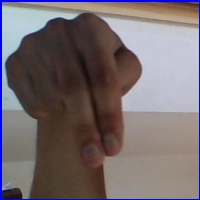
\includegraphics[width=.8\linewidth]{figures/N47_original.png}
%       \captionof{figure}{N: Failure}
%       \label{fig:N47_original}
%     \end{minipage}%
%     \begin{minipage}{.25\textwidth}
%       \centering
%       \includegraphics[width=.8\linewidth]{figures/N48.jpg}
%       \captionof{figure}{N: recognized}
%       \label{fig:test2}
%     \end{minipage}
% \end{figure}

\begin{enumerate}
    \item Does targeted data augmentation reduce confusion between certain letters more effectively than general data augmentation?
    \item To what extent does applying a \(3 \times 3\) dilation filter recover visually plausible hand landmarks in ASL Alphabet training images for which MediaPipe initially detects \textit{no\_hand}?
    \item Research Question 3
\end{enumerate}

\section{Related works}
Briefly provide an overview of previous research and studies that are relevant to your topic. Show how this project fits into the broader conversation. Highlight what has already been done / discussed. Summarize key findings, identify gaps or limitations in existing research, and explain how your project builds on or differs from past efforts. Focus on the most important and credible sources and keep your explanations clear and concise.

\section{Methods}
Describe the methods used. How it works. It can include algorithms, system descriptions, new language constructs, analyses, etc.
Provide diagrams to help in the discussion. Figure \ref{fig:one-col-figure} and Figure \ref{fig:two-col-figure} shows an example of a one-column figure and a two-column figure. 

\subsection{Image Preprocessing}

For RQ2, image preprocessing is applied as a second attempt to obtain hand landmarks from images for which MediaPipe initially returns no hand detection. Three transformations are compared: dilation, erosion and a Canny-edge overlay. Each transformation modifies the original image independently, after which the same hand detector is applied again. This comparison measures whether changing the input image allows the detector to recover a previously missed hand.

    \subsubsection{Dilation}
        Replaces a pixel value in each color channel with the highest value in its vicinity. This allows light areas to expand and contours to change.

    \subsubsection{Erosion}
    	It uses the lowest value in that area. This allows light areas to become smaller and dark areas to expand.

    \subsubsection{Canny overlay}
        Zoekt randen op basis van veranderingen in helderheid en voegt de gevonden randen toe aan de oorspronkelijke kleurenfoto. In jouw implementatie worden die randen lichter gemaakt.

% \begin{figure}
%     \centering
%     \includegraphics[width=\linewidth]{figures/example_plot.png}
%     \caption{One-column figure that explains the steps or framework of your method / model.}
%     \label{fig:one-col-figure}
% \end{figure}

% \begin{figure*}
%     \centering
%     \includegraphics[width=\linewidth]{figures/example_pipeline.png}
%     \caption{One-column figure that explains the steps or framework of your method / model.}
%     \label{fig:two-col-figure}
% \end{figure*}

\section{Experimental Results}
    \subsection{Datasets}
        Include a description of the data used, what it contains, train test splits, etc.
        \\\\
        ...
        \\\\
        
        For RQ2, we use the A-Z training images from the Kaggle ASL Alphabet dataset. This subset contains 78,000 images, with 3,000 images per letter. The additional classes \textit{space}, \textit{delete}, and \textit{nothing} are outside the scope of this experiment.
        \\\\
        All original images are first processed by MediaPipe. Images with the status \texttt{no\_hand} are selected for the recovery experiment. The supplied Kaggle test images are excluded from RQ2. This experiment evaluates hand-detection recovery within the original training images.
        \\\\
        Image N47 (Figure~\ref{fig:N47_original}) is used as a development example to inspect the effect of dilation. The complete evaluation includes N47 and images inspected during earlier development. It therefore describes the results on the full dataset, including previously examined images.
        
    \subsection{Implementation Details}
        ...
        \\\\
        ...
        \\\\
        
        MediaPipe Hand Landmarker processes each image in IMAGE mode, with both detection and presence thresholds set to 0.50. Up to two hands are detected so that multiple-hand outputs can be identified. The same model and settings are used for the original and processed images.\footnote{The detector configuration and output validation are implemented in \texttt{research/data.py}, in the \texttt{Detector} class.} The software versions, settings and checksums are recorded in \texttt{\ref{fig:preprocessing-config} settings.json} in the digital supplement for the \texttt{test\_all} run.
        \\\\
        Each image with the original status \texttt{no\_hand} is processed using three separate variants. Dilation and erosion each use a square $3 \times 3$ kernel with one iteration. Both operations are applied to the colour image at its original resolution.
        \\\\
        For the Canny-overlay variant, the image is converted to grayscale and smoothed using a $5 \times 5$ Gaussian filter. Canny edge detection uses thresholds of 50 and 150. The resulting edge map is converted to three channels and added to the original colour image, using weights of 0.25 for the edges and 1.0 for the original image.
        \\\\
        Each variant is created independently from the original image. The processed images are saved as lossless PNG files and passed to the same detector during the retry step.\footnote{The transformations are defined in the \texttt{variants} function in \texttt{research/morphology\_pilot.py}. The baseline, preprocessing and retry stages are implemented in \texttt{research/recovery\_experiment.py}.}
        \\\\
        Outputs are paired using the original image identifier. Technical recovery is defined as a transition from \texttt{no\_hand} to \texttt{ok}, requiring exactly one detected hand and successful geometric validation. For the combined result, each image is counted once if at least one variant produces \texttt{ok}. A systematic visual assessment of the recovered landmarks remains to be completed.
        \\\\
        The exported results are analysed using pandas to calculate recovery counts and percentages per preprocessing variant and per letter. Each recovery percentage uses the number of originally missed images in the corresponding group as its denominator. An image may contribute to multiple variant counts, while the combined recovery count includes each image only once.
        \\\\
        Matplotlib is used to visualise the results calculated with pandas. The figures are exported as PNG and PDF files. The underlying plotting data are saved as CSV files, together with source-file checksums and plotting-library versions, to support verification and reproduction.\footnote{The calculations and figures are generated by \texttt{experiments/hand\_detection\_recovery/plot\_results.py}.}
        
    
    \subsection{Results}
    \label{sec:rq2-results}
        Analyze and discuss your results. Table \ref{tab:example-table} shows an example of a table.
        Include plots and visualizations such as Figure \ref{fig:one-col-figure}.
        \\\\
        ...
        \\\\            
        In the baseline run, 60,251 of the 78,000 A-Z training images passed the single-hand acceptance criteria. MediaPipe returned \textit{no\_hand} detection for 17,598 images (22.56\%) and multiple hands for 151 images (0.19\%). The complete per-image detection results are available in \texttt{baseline.csv} in the digital supplement for the \texttt{test\_all} run.
        \\\\
        For the development example N47, the original image produced \textit{no\_hand} detection. After one application of $3 \times 3$ dilation, the detector returned one hand that passed geometric validation under the same confidence thresholds. The measured outcomes for this image are recorded in \texttt{n47\_example.csv}.
        \\\\
        All 17,598 initially missed images were subsequently processed using the three variants. Dilation recovered 3,560 images (20.23\%), erosion recovered 2,018 images (11.47\%), and the Canny overlay recovered 1,391 images (7.90\%). At least one variant recovered 4,799 unique images (27.27\%). Figure~\ref{fig:rq2-recovery} compares the individual recovery rates with the combined result.


        
        \begin{figure*}[h]
            \centering
            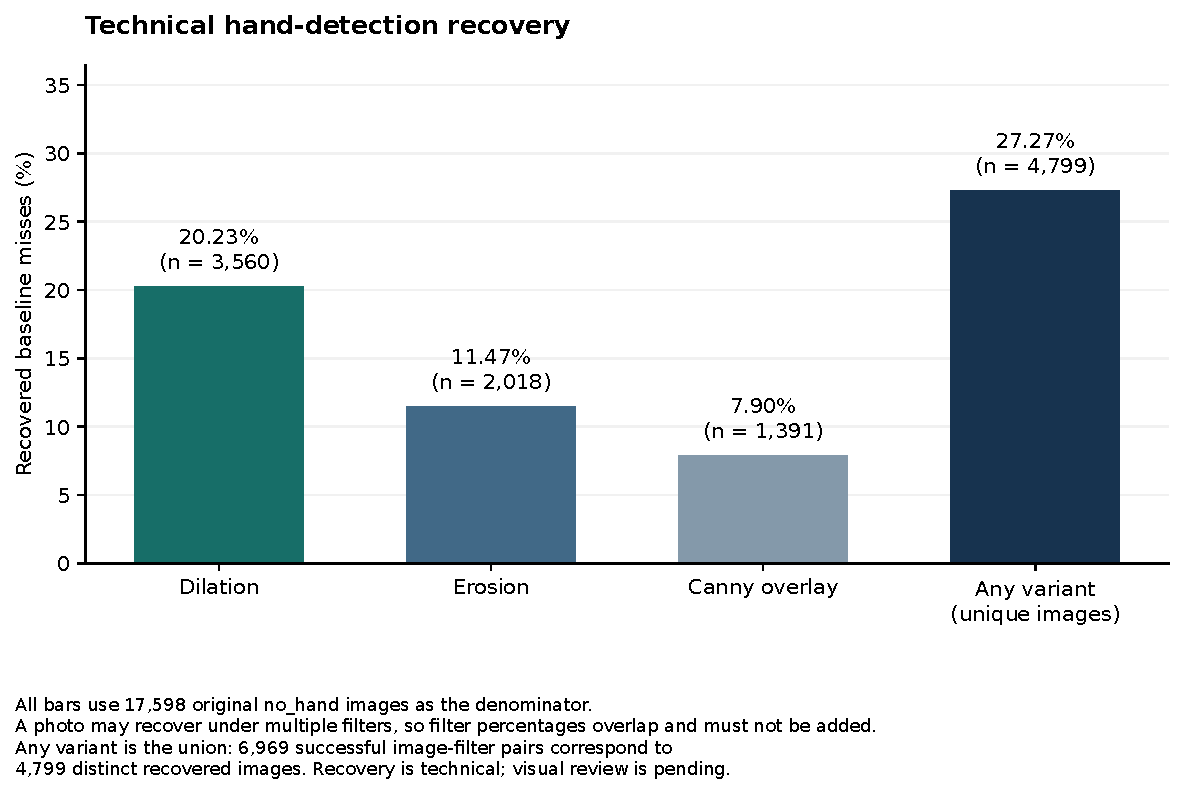
\includegraphics[width=\linewidth/2]{figures/recovery_by_variant.pdf}
            \caption{Technical recovery among the 17,598 originally missed images. Individual filter groups overlap because an image can be recovered by multiple variants. The combined result counts each recovered image once. Percentages were calculated using pandas and plotted with Matplotlib.}
            \label{fig:rq2-recovery}
        \end{figure*}
        
        The percentages for the individual variants overlap. An image recovered by both dilation and erosion contributes to both variant counts, but only once to the combined result. The three variants produced 6,969 successful image-filter pairs, corresponding to 4,799 distinct recovered images. The individual percentages therefore cannot be added to obtain the combined recovery percentage.
        \\\\
        Of the 4,799 recovered images, 3,024 were recovered by exactly one variant, 1,380 by exactly two variants, and 395 by all three variants. These counts explain the difference between the total number of successful image-filter pairs and the number of unique recovered images.
        \\\\
        After all retries, 12,799 images had no accepted detection under any variant. Of these, 12,779 images retained the status \texttt{no\_hand} under all three variants. The remaining 20 images produced another rejection status under at least one variant.
        \\\\
        The per-image outcomes and successful variants are recorded in \texttt{per\_image.csv}. Images without an accepted retry are listed in \texttt{unrecovered.csv}. Images with \texttt{no\_hand} under every variant are listed separately in \texttt{still\_no\_hand.csv}. These results quantify technical recovery. The proportion of visually plausible recoveries has not yet been established.
        \\\\
        To assess repeatability, the complete experiment was executed a second time on the same workstation using identical recorded settings, software versions and model files. Both runs produced identical detection outcomes for all 78,000 original images and identical checksums for all 52,794 processed images. The retry statuses also matched for every image and variant. For all 6,969 successful retries, the stored image and world landmark coordinates were exactly equal. Both runs recovered 4,799 unique images, corresponding to 27.27\% of the originally missed images. The comparison results and checksums of the compared output files are recorded in \texttt{\ref{fig:repeatablity} \nameref{fig:repeatablity}} in the digital supplement for the \texttt{test\_all\_repeat} run.
        
    \subsection{Discussion}
        Additionally, you can include a separate discussion section in which you summarize the results, indicate possible limitations of your work, and provide suggestions for future research.
        \\\\
        ...
        \\\\

        Dilation produced the highest technical recovery rate of the three evaluated variants. The higher combined recovery rate shows that the other variants also recovered images that dilation did not recover. However, the combined result requires trying all three variants and accepting an image when at least one attempt succeeds.
        \\\\
        The N47 example demonstrates that a small change to the input pixels can change the detection outcome while the model and thresholds remain fixed. The experiment does not establish which individual change in a contour, texture or contrast caused this response. Such explanations require further controlled comparisons and visual inspection.
        \\\\
        The results are limited to the evaluated dataset and detector configuration. N47 and earlier development images are included in the complete run, and the reported results therefore include previously examined examples. In addition, technical recovery does not establish the accuracy of the estimated hand points. A visual assessment is needed to determine whether the recovered landmarks are plausible.
        \\\\
        The agreement between the two runs supports repeatability under the recorded conditions. Repeatability across other computers, software versions or detector models was not evaluated. The coordinate comparison covers the retry detections, as landmark coordinates from the original baseline images were not retained.
        \\\\
        The contribution to RQ2 is therefore the measured technical recovery of initially missed images. Whether these recovered images improve letter recognition requires a separate training and evaluation experiment.
        
    \subsection{Citing references}
        LaTeX manages the citations for you. You simply have to add the bibtex entry for the reference in the references.bib file and you can use the citation in the paper \cite{langley00}. You can also cite multiple references in one command \cite{DudaHart2nd,Newell81,kearns89}. The bibtex entries for a paper can be obtained in websites such as google scholar or dblp.
        
        \begin{table}[h]
            \centering
            \label{tab:example-table}
            \caption{Example Table}
            \begin{tabular}{lllll}
                \toprule
                \multirow{2}{*}{Models} & \multicolumn{3}{c}{Metric 1} & Metric 2\\
                \cmidrule{2-4} \cmidrule{5-5} \\
                {} & precision & recall & F-score  & R@10 \\
                \midrule
                model 1 & 0.67  & 0.8 & 0.729  & 0.75 \\
                model 2 & 0.8 & 0.9 & 0.847 & 0.85 \\
                \bottomrule
            \end{tabular}
        \end{table}

\bibliography{references}
\bibliographystyle{icml2021}


\appendix
\section{Appendices}



\begin{figure}[H]
\centering
\begin{minipage}{0.95\linewidth}
\begin{verbatim}
{
  "source": "...ktai-hand-gesture\\data
            \\asl-alphabet-download",
  "limit": null,
  "inventory_sha256": "...",
  "images": 78000,
  "mediapipe": "0.10.35",
  "opencv": "4.14.0",
  "detector_sha256": "...",
  "detection_confidence": 0.5,
  "presence_confidence": 0.5,
  "num_hands": 2,
  "mode": "IMAGE",
  "kernel": [ 3, 3 ],
  "iterations": 1,
  "canny_thresholds": [ 50, 150 ],
  "blur": [ 5, 5 ],
  "overlay_weights": [ 1.0, 0.25 ],
  "code_hashes": {
    "data.py": "...",
    "morphology_pilot.py": "...",
    "recovery_experiment.py": "..."
  }
}
\end{verbatim}
\end{minipage}
\caption{Configuration of the image preprocessing pipeline}
\label{fig:preprocessing-config}
\end{figure}

\begin{figure}[H]
\centering
\begin{minipage}{0.95\linewidth}
\begin{verbatim}
{
  "reference": "ktai-hand-gesture\\experiments\\hand_detection_recovery\\runs\\test_all",
  "repeat": "ktai-hand-gesture\\experiments\\hand_detection_recovery\\runs\\test_all_repeat",
  "settings_equal": true,
  "changed_settings": [],
  "baseline": {
    "reference_records": 78000,
    "repeat_records": 78000,
    "different_records": 0
  },
  "processed": {
    "reference_records": 52794,
    "repeat_records": 52794,
    "different_records": 0
  },
  "retry": {
    "reference_records": 17598,
    "repeat_records": 17598,
    "different_records": 0
  },
  "summary": {
    "reference_records": 4,
    "repeat_records": 4,
    "different_records": 0
  },
  "landmarks": {
    "reference_records": 52794,
    "repeat_records": 52794,
    "records_with_coordinates": 6969,
    "different_coordinate_records": 0,
    "different_metadata_records": 0,
    "maximum_absolute_coordinate_difference": 0.0
  },
  "all_compared_outputs_equal": true,
  "evidence_sha256": {
    "reference": {
      "settings.json": "748dbe1997f11e793ef067d48342281f3a768e403a26d301f44cdc9b790a6e07",
      "baseline.csv": "2844e86d3309cc6ce6ca2915000f71b0a850e9ef8f17e42210a2b8dc766cd4c3",
      "processed.csv": "87805980df2d78ae7a2144120f01ba4a14542fc3b50a0ada4545947e8d790595",
      "per_image.csv": "79da23909a82dab478037b5f3c516a79c0d6591c0806f810f996ea18227e11e4",
      "summary.csv": "4c312ec4f3e4bb884c6e15f86dcef997815fa66f9642dda124b1d62c2315d556",
      "retry_landmarks.jsonl": "84e1273caba566c398ee1c833d5a0f7eb4ea087d2d87be459c2379c2c4457394"
    },
    "repeat": {
      "settings.json": "748dbe1997f11e793ef067d48342281f3a768e403a26d301f44cdc9b790a6e07",
      "baseline.csv": "2844e86d3309cc6ce6ca2915000f71b0a850e9ef8f17e42210a2b8dc766cd4c3",
      "processed.csv": "55c8c232a27aedac7344fec9b11eef80f76c4e2ee764f45b2c8aa5d6d98ae1f8",
      "per_image.csv": "79da23909a82dab478037b5f3c516a79c0d6591c0806f810f996ea18227e11e4",
      "summary.csv": "4c312ec4f3e4bb884c6e15f86dcef997815fa66f9642dda124b1d62c2315d556",
      "retry_landmarks.jsonl": "41513daca93729e615f589fc20c04def71e610176dfd8dc135cb782cd695f502"
    }
  },
  "scope": "Two executions on the same workstation. Baseline coordinates were not exported; coordinate comparison covers retry detections. Absolute output paths are excluded from content comparisons."
}
\end{verbatim}
\end{minipage}
\caption{Configuration of the image preprocessing pipeline}
\label{fig:repeatablity}
\end{figure}

%\subsection{Exploratory preprocessing experiments for RQ1}
...
\\\
...
\\\
...
\\\
...


%\subsection{Exploratory preprocessing experiments for RQ2}
\label{app:rq2-pilot}

\subsubsection{Provenance and purpose}
The experiments documented here were implemented and executed by the Codex assistant during the project discussion, using the locally available Kaggle ASL Alphabet images. The assistant added the baseline and pilot scripts and ran the measurements. Student reproduction and the planned visual assessment remain outstanding. These results document the development of the proposed dilation experiment.

RQ2 concerns recovery of visually plausible hand landmarks among initially missed images. The measurements below establish technical recovery. The visual plausibility of all recovered configurations has yet to be assessed using a fixed rubric. N47 and other inspected pilot images should be identified as development data when constructing a subsequent evaluation set.

\subsubsection{Fresh baseline and training}
The baseline processed 78,000 original A--Z training images, comprising 3,000 images per letter. The additional classes were excluded. MediaPipe Hand Landmarker 0.10.35 ran in IMAGE mode, with a maximum of two hands and detection and presence thresholds both set to 0.50. The model file was \texttt{models/hand\_landmarker.task}. A result received \texttt{ok} when exactly one hand was returned and the project's geometric validation passed.

\begin{table}[ht]\centering
\caption{Fresh detection outcomes on original A--Z training images.}
\label{tab:rq2-baseline}
\begin{tabular}{lrr}\toprule
Outcome & Images & Percentage\\\midrule
One valid hand (\texttt{ok}) & 60,251 & 77.245\\
Zero hands (\texttt{no\_hand}) & 17,598 & 22.562\\
Multiple hands & 151 & 0.194\\
Invalid geometry & 0 & 0.000\\\midrule
Total & 78,000 & 100.000\\\bottomrule
\end{tabular}
\end{table}

A fresh SVM letter classifier was fitted to the 60,251 accepted images using 820 Shin descriptors and 15 angle features. This produced \texttt{runs/clean\_training/asl\_clean.joblib}. Its fit has no independent test score. The recovery experiments below use the pretrained MediaPipe detector; the letter classifier does not determine whether a hand is detected.

\subsubsection{N47 development example}
The original N47 image returned \texttt{no\_hand}. One application of dilation with a square \(3\times3\) kernel changed its output to \texttt{ok} at the same detector thresholds. Erosion and the tested Canny overlay retained \texttt{no\_hand}. In separate threshold probes on the original pixels, lowering only the detection threshold to 0.49 retained \texttt{no\_hand}, while 0.45 yielded \texttt{ok}. These probes show sensitivity to both preprocessing and threshold choice.

The initial N47 probes were executed as terminal commands, and their outputs were recorded in the conversation. They were not exported as a dedicated CSV. The original-versus-dilation transition was subsequently rerun when generating the example images below. The exact internal detection score was not recorded.

\begin{figure}[ht]\centering
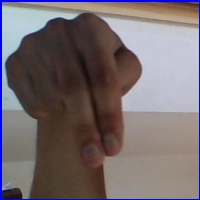
\includegraphics[height=30mm]{figures/N47_original.png}\hspace{8mm}
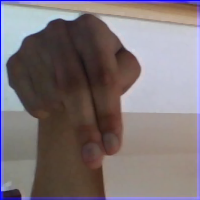
\includegraphics[height=30mm]{figures/N47_dilated.png}\hspace{8mm}
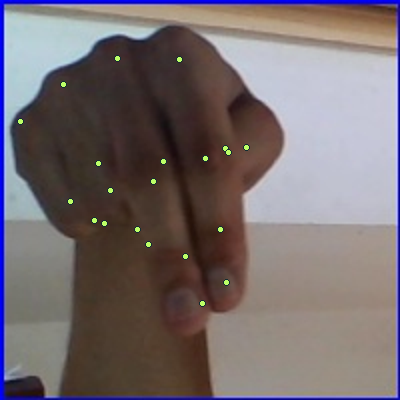
\includegraphics[height=30mm]{figures/N47_overlay.png}
\caption{N47 in its original form (left), after dilation (centre), and with recovered points overlaid on the original pixels (right). The overlay supports inspection; it does not constitute an independent landmark accuracy assessment.}
\label{fig:rq2-n47}
\end{figure}

\clearpage
\subsubsection{Letter-balanced pilot}
Using random seed 42, the pilot selected 20 initially missed and 10 initially accepted images per letter, giving 520 misses and 260 controls. The original status was rechecked before applying each transformation. Every selected photo received each of the three transformations below, with fixed detector settings.

\begin{itemize}
\item Dilation used \texttt{cv2.dilate} with a \(3\times3\) square kernel and one iteration.
\item Erosion used \texttt{cv2.erode} with the same kernel and iteration count.
\item The Canny overlay used a grayscale conversion, a \(5\times5\) Gaussian blur and Canny thresholds of 50 and 150. The three-channel edge map was added to the original RGB image with weights 0.25 and 1.0, respectively.
\end{itemize}

Image dimensions were retained, and processed arrays were supplied directly to the detector. Technical recovery means a transition from \texttt{no\_hand} to \texttt{ok}. Control loss means that an originally accepted image no longer received \texttt{ok}.

\begin{table}[ht]\centering
\caption{Exploratory pilot outcomes. Recovery denominators are 520 misses; loss denominators are 260 controls.}
\label{tab:rq2-pilot}
\begin{tabular}{lrrrr}\toprule
Transf. & Recovery & Rec (\%) & CL \footnote{Control losses} & Loss (\%)\\\midrule
Dilation & 130 & 25.00 & 6 & 2.31\\
Erosion & 64 & 12.31 & 8 & 3.08\\
Canny overlay & 49 & 9.42 & 28 & 10.77\\\bottomrule
\end{tabular}
\end{table}

The pilot gave equal weight to each letter, whereas the complete set of missed images has unequal letter counts. Its recovery percentage therefore does not directly estimate recovery across all 17,598 misses. Control losses describe applying preprocessing to already accepted images. A second-attempt procedure restricted to baseline misses bypasses these controls.

\subsubsection{Code and retained evidence}
All paths below are relative to the project root containing \texttt{app.py}.
\begin{itemize}
\item \texttt{research/data.py}, class \texttt{Detector}, defines detector settings and geometric validation.
\item \texttt{research/clean\_training.py} runs the baseline and prepares accepted inputs. The fresh classifier fit uses \texttt{--fresh-fit} in \texttt{research/live\_model.py}.
\item \texttt{research/morphology\_pilot.py} contains the transformations, deterministic sampling, paired comparisons and pilot exports.
\item \texttt{runs/clean\_training/all\_images.csv}, \texttt{no\_hand.csv} and \texttt{by\_letter.csv} contain the baseline inventory and summaries.
\item The pilot directory is \texttt{runs/clean\_training/morphology\_pilot/}. It contains \texttt{per\_foto.csv} with paired outcomes, \texttt{summary.csv} with aggregate results and \texttt{controle\_*.jpg} with overlays of recovered detections.
\end{itemize}

The pilot exports status changes and rendered overlays. A separate numerical export of all recovered landmark coordinates and a completed visual-review dataset are not yet available. The earlier \texttt{historical\_image\_audit.py} reconstructed membership in the historical accepted cohort by image ID. The fresh detector outputs listed above are the source for the present baseline counts.

\subsubsection{Reproduction and next measurement}
Run \texttt{python -m research.clean\_training --out runs/clean\_training}
from the project root with the configured Python environment. The command requires a new output directory. The existing baseline can be used to rerun \texttt{python -m research.morphology\_pilot}; this command writes to the existing pilot output paths. Preserve the original evidence before rerunning it.

A subsequent study should freeze the transformation and visual rubric, identify the development-image exclusions, and report technical and visually plausible recovery with the same eligible-image denominator. The exploratory outcomes in this appendix can motivate that design.


%\subsection{Exploratory preprocessing experiments for RQ30}
...
\\\
...
\\\
...
\\\
...


\end{document}

